Este capítulo é dedicado ao desenvolvimento do segundo algoritmo de \textit{Data Augmentation}, onde são geradas as amostras de voz 
reverberadas em campo-distante (AVCDs) usando: amostras de voz anecóicas (AVAs), RIRSM, sinais de ruído pontuais (SRPs) e de fundo (SRFs).

\begin{figure} [H]
    \centering
    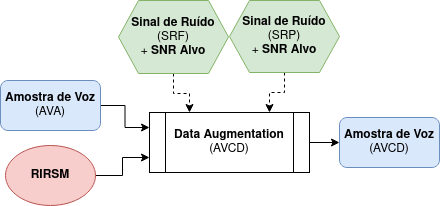
\includegraphics[scale=0.65]{flow-voz-aug.png}
    \caption{Fluxo de procedimentos para gerar a AVCD.} 
    \label{fig:flow-voz-rev}
\end{figure}

Este trabalho é uma implementação do método de DA proposto no artigo \cite{Speech_Rec}. A Figura \ref{fig:flow-voz-rev} especifica 
o fluxo de procedimentos implantados por este algoritmo, onde o SRP, SRF e SNR alvos são aleatoriamente escolhidos, 
dentro de uma base de dados de ruídos e uma faixa de valores definidas pelo usuário, que determinam as características da AVCD. 

\section{Simulação de fala em campo distante} 

Sinais de voz em campo-distante são tipicamente compostos por uma combinação de VR, SRP (assumindo que a fonte do ruído pontual encontra-se 
no mesmo ambiente da VR) e SRF (assumindo que o ruído de fundo não é afetado pelo modelo acústico do ambiente).
É possível modelar uma AVCD conforme a equação

\begin{equation} \label{eqn:AVCD-model}
    S_{cd}[t] = S_a[t] \ast h[t] + \sum_i n_{pi}[t] \ast h[t] + n_f[t]
    ,
\end{equation}

\noindent
onde $S_{cd}[t]$ representa a AVCD, $S_a[t]$ a AVA, $h[t]$ a RIR, $n_{pi}[t]$ o i-ésimo SRP e $n_f[t]$ o SRF.
Neste trabalho, diferente da implementação do algoritmo em \cite{Speech_Rec}, é considerado apenas uma única RIR
para gerar a AVCD, ou seja, os ruídos pontuais são convoluídos com a mesma RIR que é usada para a fonte de voz.

No Algoritmo \ref{alg:AVCD-gen} descreve-se o procedimento que é usado para gerar sinais de voz em campo-distante simulados. 
\bigbreak
\bigbreak

\begin{algorithm} [H] 
    \caption{Procedimentos para gerar AVCD}
    \label{alg:AVCD-gen}

    \KwIn{$fl_p$ : Flag de inclusão de ruído pontual} 
    \KwIn{$fl_g$ : Flag de inclusão de ruído de fundo} 
    \KwIn{$m$ : Quantidade de ruídos pontuais} 
    \KwIn{$SNR_{up}$ : Limite superior de SNR} 
    \KwIn{$SNR_{dw}$ : Limite inferior de SNR} 

    $S_r[t] \gets S_a[t] \ast h[t]$ : Convolução da RIR com AVA

    \If{$fl_p = true$}
    {
        \For{$i = 1$ até $m$}
        {
            Escolha aleatória de um ruído pontual $n_{pi}[t]$ da biblioteca de ruído. \\
            Escolha aleatória de uma SNR Alvo $SNR_t$ compreendida dentro do intervalo $[SNR_{dw},SNR_{up}]$. \\
            Dedução do fator $\alpha$ a partir da $SNR_t$ para corrigir a intensidade de $n_{pi}[t]$. \\
            Escolha aleatória de offset $o_t$ compreendida dentro do intervalo $(0,\text{duração(t)})$. \\
            $S_r[t] \gets S_r[t] + \alpha \text{ offset}(n_{pi}[t] \ast h[t], o_t)$ : Adição de SRP na AVR.
        }
    }
    \If{$fl_g = true$}
    {
        Escolha aleatória de um ruído de fundo $n_f[t]$ da biblioteca de ruído. \\
        Escolha aleatória de uma SNR Alvo $SNR_t$ compreendida dentro do intervalo $[SNR_{dw},SNR_{up}]$. \\
        Dedução do fator $\alpha$ a partir da $SNR_t$ para corrigir a intensidade de $n_f[t]$. \\
        Estender ou encurtar $n_f[t]$ até que $\text{duração }(n_f[t]) = \text{duração}(S_r[t])$
        $S_r[t] \gets S_r[t] + \alpha n_f[t]$ : Adição de SRF na AVR.
    }

\end{algorithm}
%\bigbreak
%\bigbreak
\pagebreak


Neste trabalho, o algoritmo de geração de AVCD usa as RIRSMs geradas através do primeiro algoritmo, diferente do que foi implantado
em \cite{Speech_Rec}, onde foram geradas RIRs de forma completamente digital \cite{RIR_sim_image}, ou seja, sem usar RIRs reais 
como base para \textit{Data Augmentation}.
Nota-se também que o algoritmo permite habilitar ou não o uso de cada tipo de ruído para que possa aumentar a variedade de dados gerados, além
de acomodar mais propósitos de treinamentos de \textit{Deep Learning}.

A Figura \ref{fig:voice-sample} exibe uma amostra de voz anecóica que foi usada para gerar os próximos exemplos de aplicação
do algoritmo. É feita uma comparação entre a convolução da AVA com a RIRO e com a RIRSM, representadas nas Figuras \ref{fig:voice-aug-riro} e 
\ref{fig:voice-aug-rirsm}, respectivamente; pode-se notar que a convolução com a RIRSM causa menos modificações no formato do sinal de voz original 
comparado à RIRO, uma vez que a primeira DA foi configurada para simular um ambiente menos reverberante, partindo dos parâmetros $DRR=-4$ e $T60=1,38$ s
na RIRO para $DRR=10$ e $T60=0,50$ s na RIRSM.

\begin{figure} [H]
    \centering
    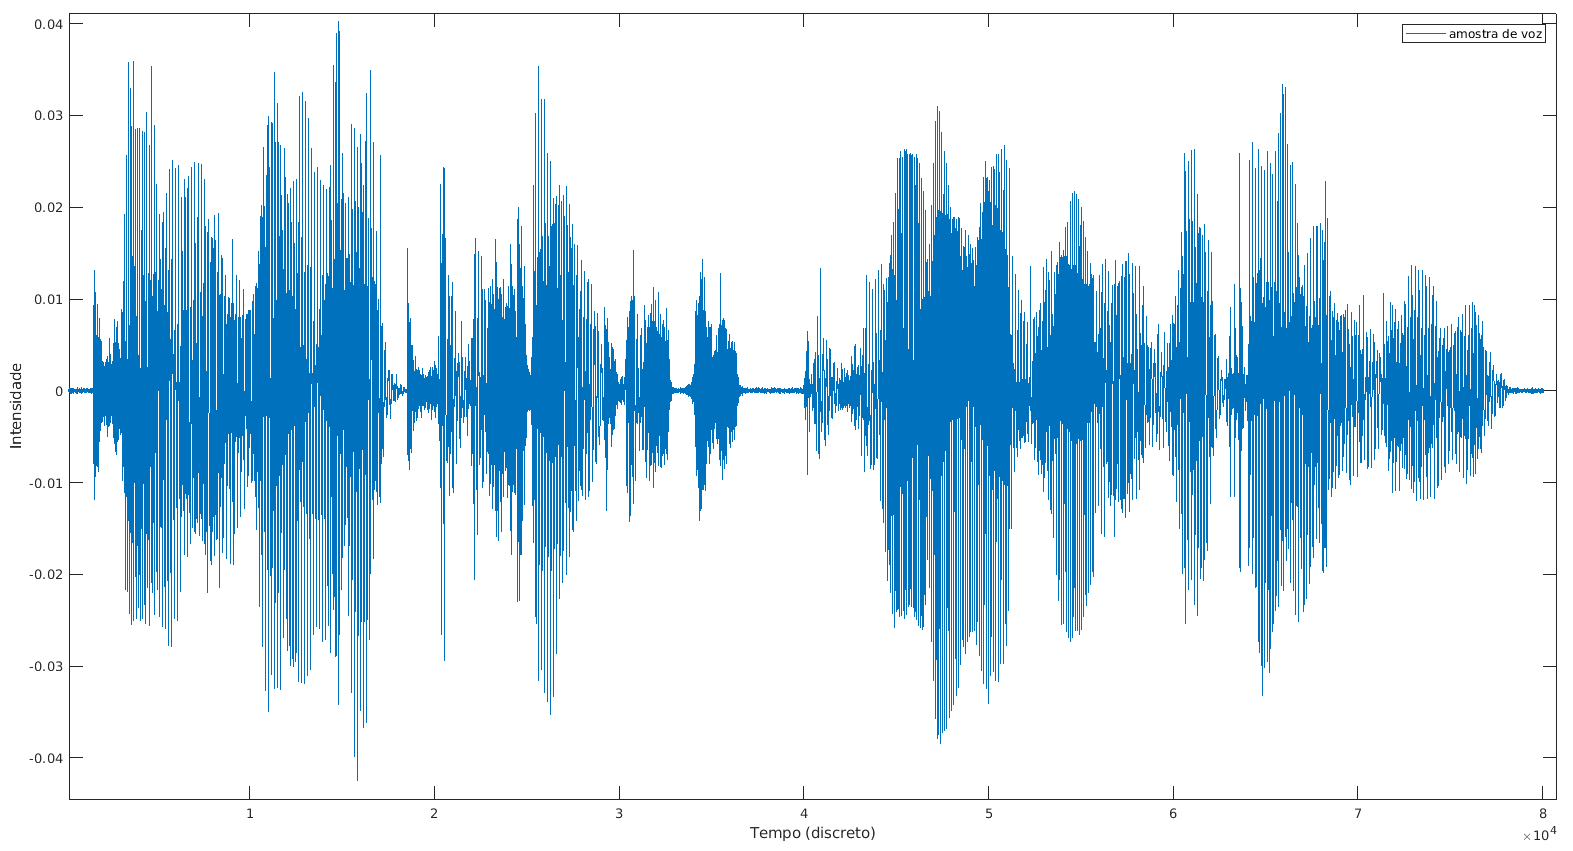
\includegraphics[scale=0.3]{voice-sample.png}
    \caption{Exemplo de amostra de voz anecóica.}
    \label{fig:voice-sample}
\end{figure} 

\begin{figure} [H]
    \centering
    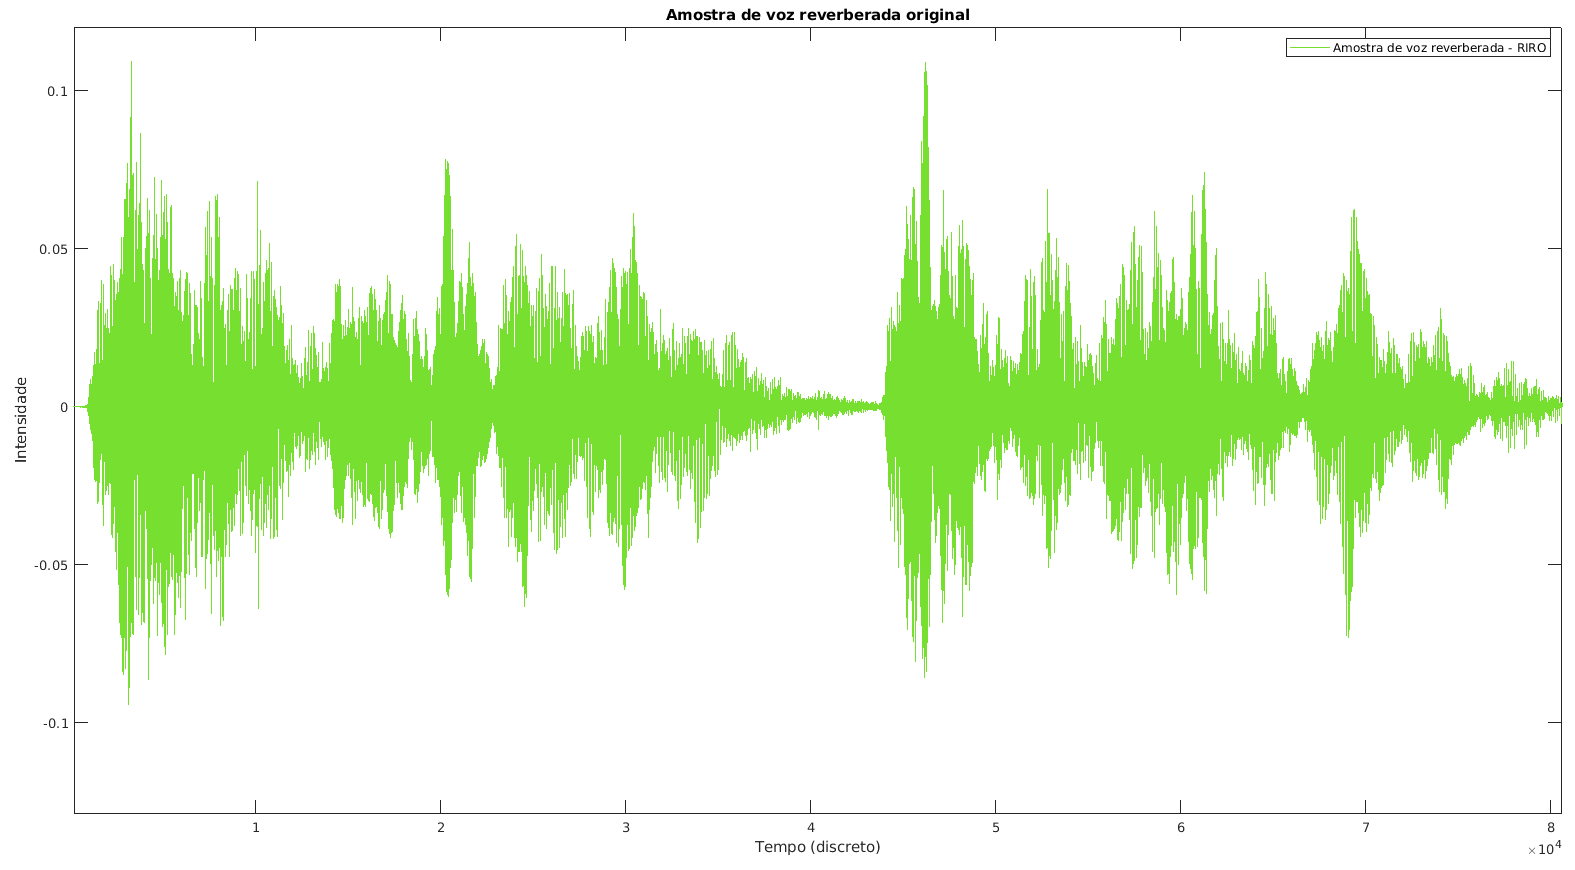
\includegraphics[scale=0.3]{voice-aug-riro.png}
    \caption{Exemplo de amostra de voz reverberante, convoluída com uma RIRO, onde $DRR = -4$ e $T60=1,38$ s.}
    \label{fig:voice-aug-riro}
\end{figure} 

\begin{figure} [H]
    \centering
    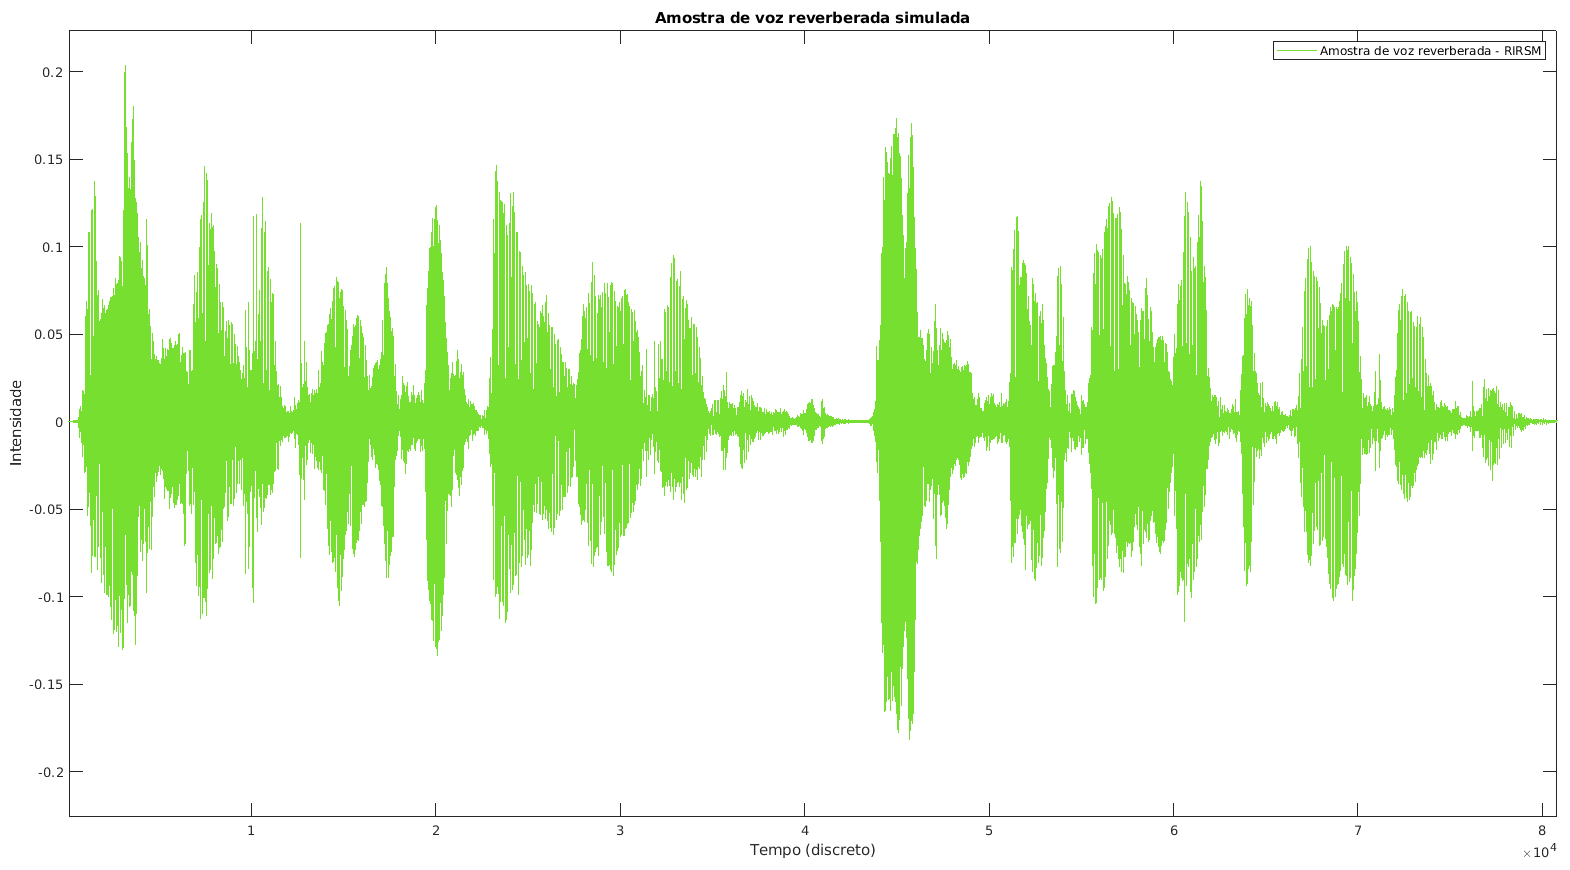
\includegraphics[scale=0.3]{voice-aug-rirsm.png}
    \caption{Exemplo de amostra de voz reverberante, convoluída com uma RIRSM, onde $DRR = 10$ e $T60=0,50$ s.}
    \label{fig:voice-aug-rirsm}
\end{figure} 

A partir da RIRSM usada nesta aplicação, foram gerados dois exemplos de AVCDs, representadas nas Figuras \ref{fig:voice-noise-14snr} e 
\ref{fig:voice-noise-4snr}, esta com $SNR = 4$ e aquela com $SNR = 14$. Conforme o esperado, observa-se que a AVCD com o menor SNR
possui ruídos claramente mais acentuados comparada à AVCD com o maior SNR.

\begin{figure} [H]
    \centering
    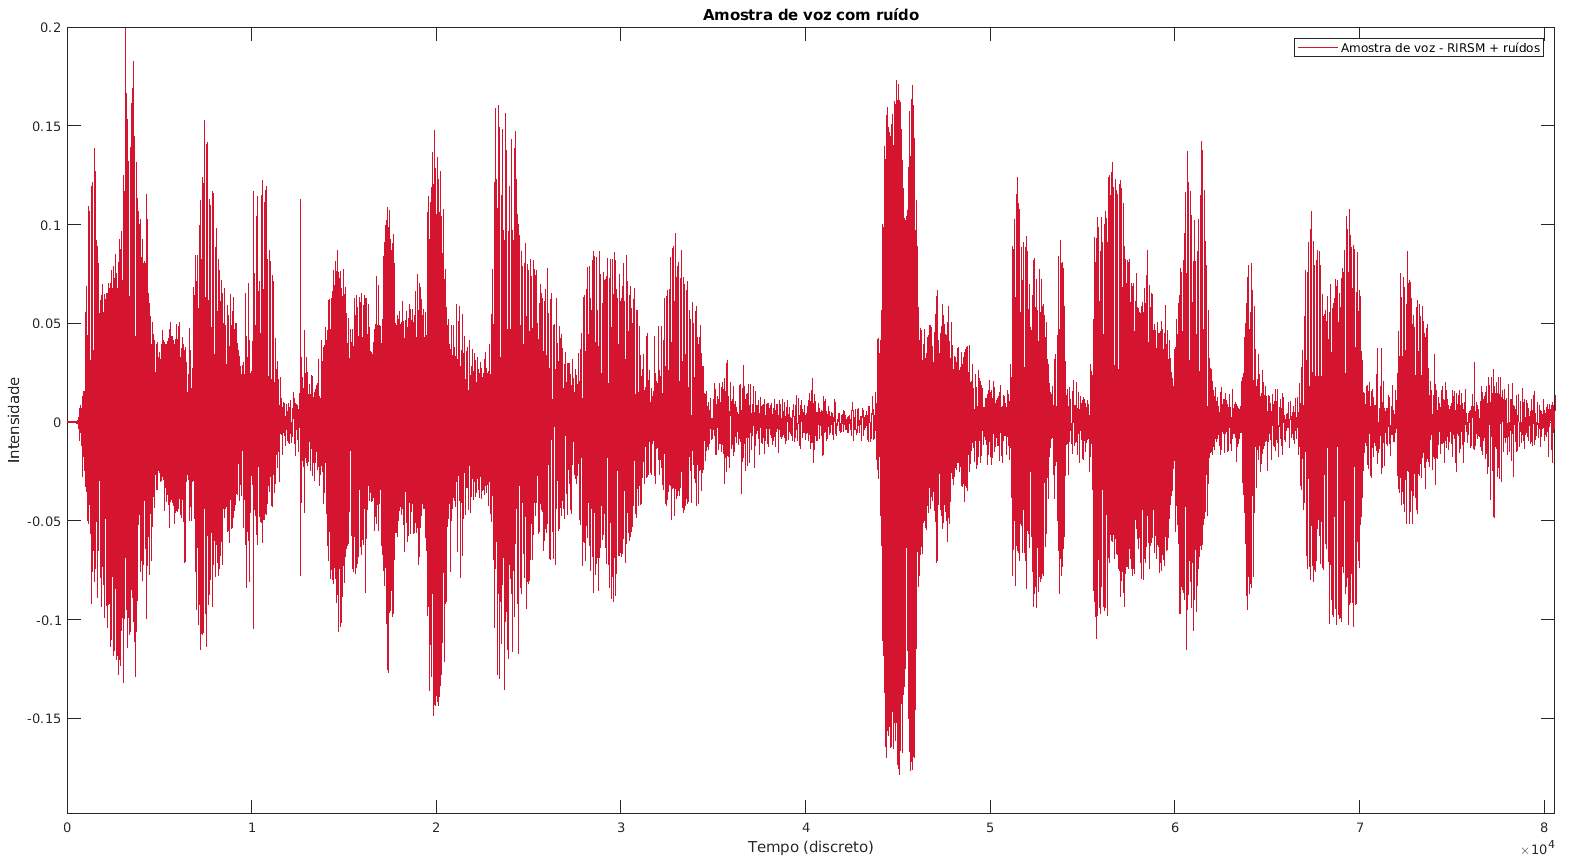
\includegraphics[scale=0.3]{voice-noise-14snr.png}
    \caption{Exemplo de amostra de voz em campo distante com $SNR = 14$, representada pela voz reverberada mais os ruídos adicionados pelo segundo método de DA.}
    \label{fig:voice-noise-14snr}
\end{figure} 

\begin{figure} [H]
    \centering
    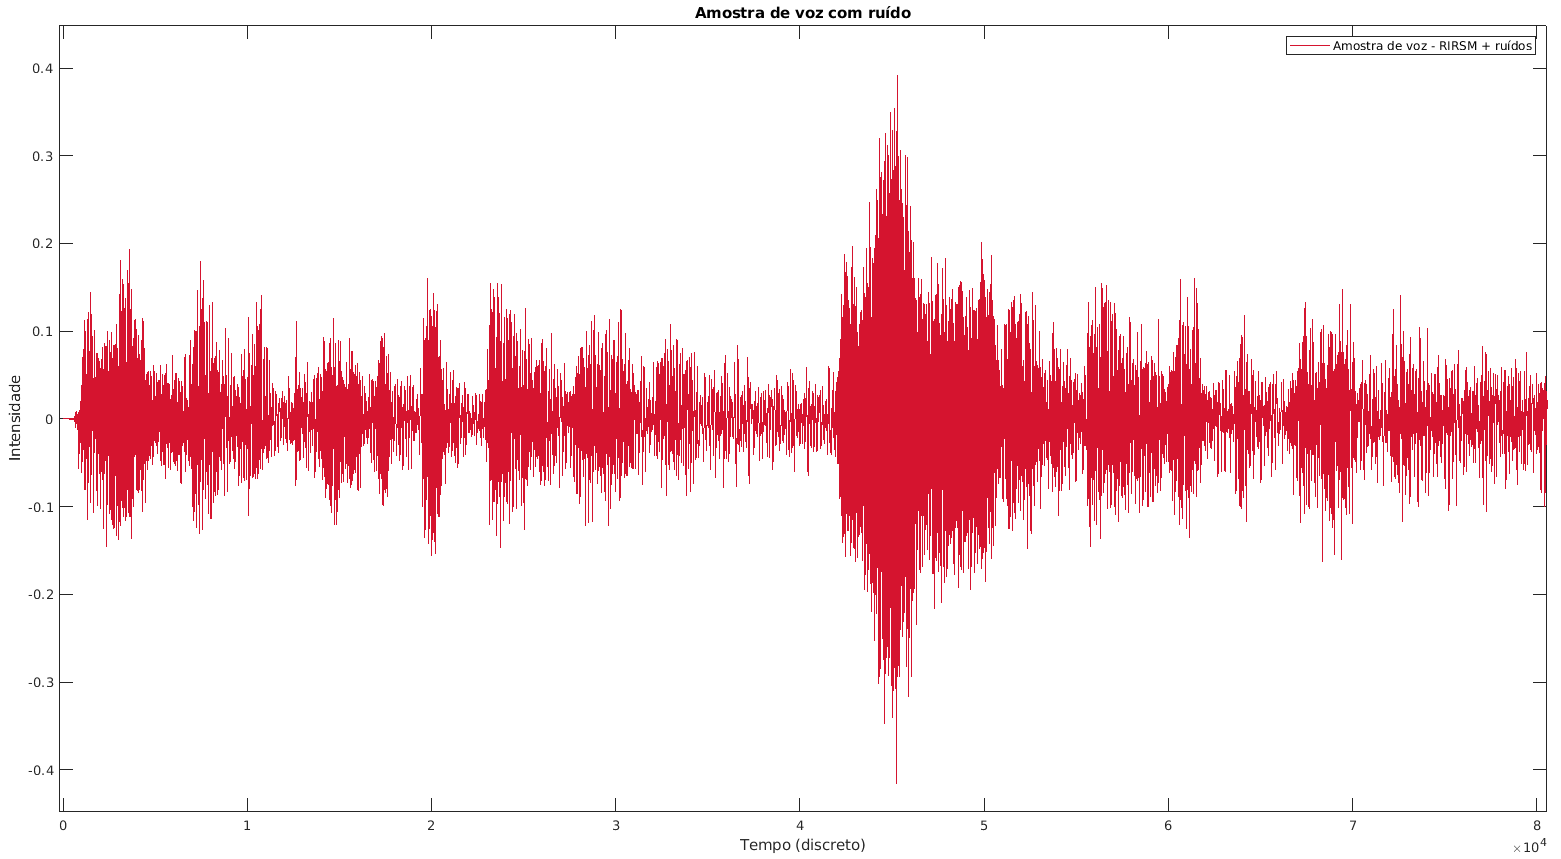
\includegraphics[scale=0.3]{voice-noise-4snr.png}
    \caption{Exemplo de amostra de voz em campo distante com $SNR = 4$, representada pela voz reverberada mais os ruídos adicionados pelo segundo método de DA.}
    \label{fig:voice-noise-4snr}
\end{figure} 